\documentclass[english, a4paper]{article}

\usepackage[T1]{fontenc}    % Riktig fontencoding
\usepackage[utf8]{inputenc} % Riktig tegnsett
\usepackage{babel}          % Ordelingsregler, osv
\usepackage{graphicx}       % Inkludere bilder
\usepackage{booktabs}       % Ordentlige tabeller
\usepackage{url}            % Skrive url-er
\usepackage{textcomp}       % Den greske bokstaven micro i text-mode
\usepackage{units}          % Skrive enheter riktig
\usepackage{float}          % Figurer dukker opp der du ber om
\usepackage{lipsum}         % Blindtekst
\usepackage{subcaption} 
\usepackage{color}
\usepackage{amsmath}  
\usepackage{hyperref}
\usepackage{pagecolor}
\usepackage{minted}
\usepackage{braket} 
\usepackage{multicol}
\usepackage{listings}    %Add source code
\usepackage{amsfonts}
\usepackage{setspace}
\usepackage[cm]{fullpage}		% Smalere marger.
\usepackage{verbatim} % kommentarfelt.
\usepackage{tabularx}
\setlength{\columnseprule}{1pt}	%(width of separationline)
\setlength{\columnsep}{1.0cm}	%(space from separation line)
\newcommand\lr[1]{\left(#1\right)} 
\newcommand\bk[1]{\langle#1\rangle} 
\newcommand\uu[1]{\underline{\underline{#1}}} % Understreker dobbelt.
\definecolor{qc}{rgb}{0,0.4,0}
\definecolor{LightBlue}{rgb}{0.8, 0.8, 0.9}
\hypersetup{
	colorlinks,
	linkcolor={red!30!black},
	citecolor={blue!50!black},
	urlcolor={blue!80!black}
}
% JF i margen
\makeatletter
\renewcommand{\subsubsection}{\@startsection{subsubsection}{3}{0pt}%
{-\baselineskip}{0.5\baselineskip}{\bf\large}}
\makeatother
\newcommand{\jf}[1]{\subsubsection*{JF #1}\vspace*{-2\baselineskip}}

\newcommand{\bm}[1]{\mathbf{#1}}

% Skru av seksjonsnummerering (-1)
\setcounter{secnumdepth}{3}

\begin{document}
%\pagecolor{black!50!}
\renewcommand{\figurename}{Figure}
% Forside
\begin{titlepage}
\begin{center}

\textsc{\Large FYS4411 - Computational quantum mechanics }\\[0.5cm]
\textsc{\Large Spring 2016}\\[1.5cm]
\rule{\linewidth}{0.5mm} \\[0.4cm]
{ \huge \bfseries  Project 1;\\ Variational Monte Carlo Studies of Bosonic systems}\\[0.10cm]
\rule{\linewidth}{0.5mm} \\[1.5cm]
\textsc{\Large temporary report}\\[1.5cm]


% Av hvem?
\begin{minipage}{\textwidth}
\begin{minipage}{0.49\textwidth}
    \begin{center} \large
        Sean Bruce Sangolt Miller\\
        {\footnotesize s.b.s.miller@fys.uio.no}
    \end{center}
\end{minipage}
\quad
\begin{minipage}{0.49\textwidth}
    \begin{center} \large
        Filip Henrik Lasren\\
        {\footnotesize filiphenriklarsen@gmail.com}
    \end{center}
\end{minipage}
\end{minipage}
\vfill

% Dato nederst
\large{Date: \today}

\end{center}
\end{titlepage}
%%%%%%%%%%%%%%%%%%%%%%%%%%%%%%%%%%%

\begin{abstract}
 Some text that is abstact
\end{abstract}


%%%%%%%%%%%%%%%%%%%%%%%%%%%%%%%%%%%
\pagenumbering{gobble}% Remove page numbers (and reset to 1)
\tableofcontents
\newpage
\pagenumbering{arabic}% Arabic page numbers (and reset to 1)
%\begin{multicols*}{2}


\section{Introduction}


\section{Theory and methods}

A brief on VMC

\subsection{Preliminary derivations}

\subsubsection{Simplified problem}
The local energy is defined as:

\begin{equation}
    E_L({\bf R})=\frac{1}{\Psi_T({\bf R})}H\Psi_T({\bf R}),
    \label{eq:locale}
\end{equation}

As a first approximation, it is assumed there is no interaction term in the Hamiltonian, which means the hard sphere bosons have no physical size (the hard-core diameter is zero). It is also assumed that no magnetic field is applied to the bosonic gas, leaving a perfectly spherically symmetrical harmonic trap. Inserting this new Hamiltonian into the local energy gives:

\begin{equation}
  E_L({\bf R})=\frac{1}{\Psi_T({\bf R})}\sum_i^N \left(
  \frac{-\hbar^2}{2m}
  \nabla_{i}^2 +
  \frac{1}{2}m\omega_{ho}^2r_i^2\right)\Psi_T({\bf R})
  \label{eq:localeInsertH}
\end{equation}

The potential term is trivial since this is a scalar, i.e. the denominator will cancel the wavefunction. A more challenging problem is to find an expression for $\nabla^2_i\Psi_T({\bf R})$. The trial wavefunction shown in equation (...), with the aforementioned approximations, is:

\begin{equation}
 \Psi_T({\bf R}) = \prod_i e^{-\alpha r_i^2}	\label{wavefunction_a}
\end{equation}

where $\alpha$ is the variational parameter for VCM. The first derivative is:

\begin{align}
 \nabla_j\prod_i e^{-\alpha r_i^2} 
 &= -2\alpha \bm{r}_j e^{-\alpha r_j^2} \prod_{i \neq j} e^{-\alpha r_i^2}\\
 &= -2\alpha \bm{r}_j  \prod_i e^{-\alpha r_i^2}.
 \label{E_L_first_derivative}
\end{align}

The second derivative then follows:

\begin{align}
 \nabla_j^2 \prod_i e^{-\alpha r_i^2} 
 &= \nabla_j \lr{-2\alpha \bm{r}_j  \prod_i e^{-\alpha r_i^2}}\\
 &= \lr{4\alpha^2 r_j^2 - 2d\alpha}  \prod_i e^{-\alpha r_i^2}.	\label{simpleLaplacian}
\end{align}

where $d$ is the number of dimensions. Inserting this into back into the local energy (equation \eqref{eq:localeInsertH}), the final expression can be derived:

\begin{align}
\begin{split}
 E_L({\bf R}) &= \frac{1}{\Psi_T({\bf R})}\sum_i^N \lr{
	 \frac{-\hbar^2}{2m}
	 \nabla_{i}^2 +
	\frac{1}{2}m\omega_{ho}^2r^2}\Psi_T({\bf R})\\
    &= \sum_{i=1}^N\left[\frac{-\hbar^2}{2m}\lr{4\alpha^2 r_i^2 - 2d\alpha} + \frac{1}{2}m\omega_{ho}^2r_i^2\right] \label{SimpleLocalEnergies}
\end{split}
\end{align}



The drift force (quantum force), still with the approximations above, is defined by:

\begin{equation}
	F = \frac{2\nabla\Psi_T}{\Psi_T}
\end{equation}

The gradient here is defined as

\begin{equation*}
	\nabla \equiv \lr{\nabla_1,\nabla_2,\ldots,\nabla_N}
\end{equation*}

i.e. a vector of dimension $Nd$. The gradient with respect to a single particle's position is already given in equation \ref{E_L_first_derivative}, so it's not too hard to realise:

\begin{align*}
	F &= \frac{-4\alpha}{\Psi_T}\lr{\bm{r}_1,\bm{r}_2,\ldots,\bm{r}_N}\Psi_T\\
	&= -4\alpha\lr{\bm{r}_1,\bm{r}_2,\ldots,\bm{r}_N}
\end{align*}


\subsubsection{Full problem}

The full local energy\footnote{The "full local energy" means not making any assumptions on the particle interactions or the potential.} is a bit more tedious to derive. The first step is to rewrite the trial wavefunction to the following form:

\begin{equation}
	\Psi_T(\bm{R}) = \prod_{i} \phi(\bm{r}_i)e^{\sum_{i'<j'}u(r_{i'j'})}
\end{equation}

where, in order for this to fit with the previous wavefunction, $u(r_{ij}) \equiv \ln[f(r_{ij})]$ and $\phi(\bm{r}_i) \equiv g(\alpha,\beta,\bm{r}_i)$. The gradient with respect to the $k$-th coordinate set is:

\begin{align}
	\nabla_k\Psi_T &= \nabla_k\prod_i \phi(\bm{r}_i)e^{\sum_{i'<j'}u(r_{i'j'})}\\
	&= \nabla_k\phi_k\left[\prod_{i\neq k} \phi(\bm{r}_i)e^{\sum_{i'<j'}u(r_{i'j'})}\right] + \left[\prod_i \phi(\bm{r}_i)e^{\sum_{i'<j'}u(r_{i'j'})}\nabla_k\left(\sum_{i''<j''}u_{i''j''} \right)\right]\\
	&= \nabla_k\phi_k\left[\prod_{i\neq k} \phi(\bm{r}_i)e^{\sum_{i'<j'}u(r_{i'j'})}\right] + \left[\prod_i \phi(\bm{r}_i)e^{\sum_{i'<j'}u(r_{i'j'})}\left(\sum_{i''<j''}\nabla_ku_{i''j''} \right)\right]
\end{align}

The function $u_{ij}$ is symmetric under permutation $i \leftrightarrow j$, as one can see from the definitions of $u_{ij}$ and $f(r_{ij})$. Therefore, the last sum above can have a different indexing: All terms without an index $k$, will give zero when taking the derivative $\nabla_k$, so only $i=k$ or $j=k$ remains (remember $i \neq j$). Due to the symmetry of $u_{ij}$, one can simply always say $i=k$ and let $j$ be the summation index:

\begin{equation}
	\nabla_k\Psi_T = \nabla_k\phi_k\left[\prod_{i\neq k} \phi(\bm{r}_i)e^{\sum_{i'<j'}u(r_{i'j'})}\right] + \left[\prod_i \phi(\bm{r}_i)e^{\sum_{i'<j'}u(r_{i'j'})}\left(\sum_{j''\neq k}\nabla_ku_{kj''} \right)\right]
	\label{eq:grad}
\end{equation}

The second derivative now becomes (where $\nabla_k$ only acts on the first parenthesis to its right):

\begin{align*}
	\nabla_k^2\Psi_T &= (\nabla_k^2\phi_k)\left[\prod_{i\neq k} \phi(\bm{r}_i)e^{\sum_{i'<j'}u(r_{i'j'})}\right] + (\nabla_k\phi_k) \left[\prod_{i\neq k}\phi(\bm{r}_i)\nabla_ke^{\sum_{i'<j'}u(r_{i'j'})}\right]\\
	&\:\:\:\:\:\: + \left[\nabla_k\left(\prod_i \left(\phi(\bm{r}_i)\right)e^{\sum_{i'<j'}u(r_{i'j'})}\right)\left(\sum_{j''\neq k}\nabla_ku_{kj''} \right)\right]\\
	&\:\:\:\:\:\: + \left[\prod_i \phi(\bm{r}_i)e^{\sum_{i'<j'}u(r_{i'j'})}\left(\sum_{j''\neq k}\nabla_k^2u_{kj''} \right)\right]
\end{align*}

While a bit of a nuisance to read, the expression above is simply the product rule for $\nabla_k(\nabla_k\Psi_T)$. Written in terms of $\Psi_T$, the above can be a bit simplified\footnote{For the more mathematically concerned nitpicker, the product symbol only runs over the functions $\phi(\bm{r}_i))$, not the following exponential. This is easy to realise by recalling how $\Psi_T$ was defined, and is important to know when inserting $\Psi_T$ as done now.}:

\begin{align*}
	\nabla_k^2\Psi_T &= (\nabla_k^2\phi_k)\frac{\Psi_T}{\phi(\bm{r}_k)} + (\nabla_k\phi_k) \left[\prod_{i\neq k}\phi(\bm{r}_i)\nabla_ke^{\sum_{i'<j'}u(r_{i'j'})}\right]\\
	&\:\:\:\:\:\: + \left[\left(\nabla_k\Psi_T\right)\left(\sum_{j''\neq k}\nabla_ku_{kj''} \right)\right]\\
	&\:\:\:\:\:\: + \left[\Psi_T\left(\sum_{j''\neq k}\nabla_k^2u_{kj''} \right)\right]
\end{align*}

The second term above is equal to the second term in equation \ref{eq:grad}, divided by $\phi(\bm{r}_k)$. Furthermore, the gradient $\nabla_k\Psi_T$ is already calculated above, and in terms of $\Psi_T$ is:

\begin{equation}
	\nabla_k\Psi_T = \frac{\Psi_T}{\phi(\bm{r}_k)}\nabla_k\phi_k + \Psi_T\left(\sum_{j''\neq k}\nabla_ku_{kj''} \right)
\end{equation}

Inserting all this back into the second derivative yields:

\begin{align*}
	\nabla_k^2\Psi_T &= (\nabla_k^2\phi_k)\frac{\Psi_T}{\phi(\bm{r}_k)} + (\nabla_k\phi_k) \left[\frac{\Psi_T}{\phi(\bm{r}_k)}\left(\sum_{j''\neq k}\nabla_ku_{kj''} \right)\right]\\
	&\:\:\:\:\:\: + \left[\frac{\Psi_T}{\phi(\bm{r}_k)}\nabla_k\phi_k + \Psi_T\left(\sum_{j''\neq k}\nabla_ku_{kj''} \right)\right]\left(\sum_{j''\neq k}\nabla_ku_{kj''} \right)\\
	&\:\:\:\:\:\: + \left[\Psi_T\left(\sum_{j''\neq k}\nabla_k^2u_{kj''} \right)\right]
\end{align*}

Giving:

\begin{align*}
	\frac{1}{\Psi_T}\nabla_k^2\Psi_T &= (\nabla_k^2\phi_k)\frac{1}{\phi(\bm{r}_k)} + (\nabla_k\phi_k) \left[\frac{1}{\phi(\bm{r}_k)}\left(\sum_{j''\neq k}\nabla_ku_{kj''} \right)\right]\\
	&\:\:\:\:\:\: + \left[\frac{1}{\phi(\bm{r}_k)}\nabla_k\phi_k + \left(\sum_{j''\neq k}\nabla_ku_{kj''} \right)\right]\left(\sum_{j''\neq k}\nabla_ku_{kj''} \right)\\
	&\:\:\:\:\:\: + \sum_{j''\neq k}\nabla_k^2u_{kj''}
\end{align*}

Which can be rewritten to:

\begin{align}
	\frac{1}{\Psi_T}\nabla_k^2\Psi_T &= \frac{\nabla_k^2\phi_k}{\phi(\bm{r}_k)} + \frac{2\nabla_k\phi_k}{\phi(\bm{r}_k)}\left(\sum_{i\neq k}\nabla_ku_{ki} \right) + \left(\sum_{j\neq k}\nabla_ku_{kj} \right)^2 + \sum_{l\neq k}\nabla_k^2u_{kl}
\end{align}

The gradients $\nabla_k u_{ki}$ can be rewritten using partial differentiation (where $r_{k,i}$ is coordinate $i$ of $\bm{r}_k$):

\begin{align*}
	\nabla_k u_{ki} &= \left(\frac{\partial}{\partial r_{k,1}}, \frac{\partial}{\partial r_{k,2}}, \ldots\right)u_{ki}\\
	&= \frac{\partial u_{ki}}{\partial r_{ki}}\left(\frac{\partial r_{ki}}{\partial r_{k,1}}, \frac{\partial r_{ki}}{\partial r_{k,2}}, \ldots\right)\\
	&= \frac{\partial u_{ki}}{\partial r_{ki}}\left( \frac{\partial}{\partial r_{k,1}}\left(\sqrt{\left[(r_{k,1}-r_{i,1})\hat{e}_1 + \ldots\right]^2}\right), \ldots \right)\\
	&= \frac{\partial u_{ki}}{\partial r_{ki}}\left(\frac{r_{k,1} - r_{i,1}}{r_{ki}}, \ldots \right)\\
	&= \frac{\partial u_{ki}}{\partial r_{ki}}\frac{\bm{r}_k - \bm{r}_i}{r_{ki}}\\
	&= \frac{\bm{r}_k - \bm{r}_i}{r_{ki}} u_{ki}' \:\:,\:\:  u_{ki}'\equiv \frac{\partial u_{ki}}{\partial r_{ki}}
\end{align*}

While the second derivative of $u_{ki}$ is:

\begin{align*}
	\nabla_k^2 u_{ki} &= \nabla_k(\nabla_ku_{ki})\\
	&= u_{ki}'\nabla_k\left(\frac{\bm{r}_k - \bm{r}_i}{r_{ki}}\right) + \frac{\bm{r}_k - \bm{r}_i}{r_{ki}}\nabla_k u_{ki}'\\
	&= u_{ki}' \left(\frac{d}{r_{ki}} - \frac{r_{k,1}-r_{i,1}}{r_{ki}^3} - \frac{r_{k,2}-r_{i,2}}{r_{ki}^3} - \ldots\right) + \frac{\bm{r}_k - \bm{r}_i}{r_{ki}}\cdot\frac{\bm{r}_k - \bm{r}_i}{r_{ki}} u_{ki}''\\
	&= \frac{u_{ki}'}{r_{ki}} \left(d - \frac{r_{k,1}-r_{i,1}}{r_{ki}^2} - \frac{r_{k,2}-r_{i,2}}{r_{ki}^2} - \ldots\right) + u_{ki}\\
	&= \frac{u_{ki}'}{r_{ki}} \left(d - 1\right) + u_{ki}
\end{align*}

where $d$, as earlier, is the number of dimensions present, which in our world is usually $d=3$. Finally, this gives:

\begin{align}
\frac{1}{\Psi_T}\nabla_k^2\Psi_T &= \frac{\nabla_k^2\phi_k}{\phi(\bm{r}_k)} + \frac{2\nabla_k\phi_k}{\phi(\bm{r}_k)}\left(\sum_{i\neq k} \frac{\bm{r}_k - \bm{r}_i}{r_{ki}} u_{ki}' \right) + \sum_{i,j\neq k}\frac{(\bm{r}_k - \bm{r}_i)(\bm{r}_k - \bm{r}_j)}{r_{ki}r_{kj}}u_{ki}'u_{kj}' + \sum_{i\neq k} u_{ki}'' + \frac{u_{ki}'}{r_{ki}} \left(d - 1\right)
\label{eq:full_second_derivative}
\end{align}

As the exact forms of $\phi_k$ and $u_{ki}$ are known, this can be written to a more recognisable, and calculable, expression. However, this expression will be quite long, so only the necessary variables will be derived. Inserting them into equation \ref{eq:full_second_derivative} is trivial. The $u_{ki}$ derivatives are:

\begin{equation}
	\frac{\partial u_{ki}}{\partial r_{ki}} = \frac{\partial}{\partial r_{ki}}\left(\ln\left[1-\frac{a}{r_{ki}}\right]\right) = \frac{a}{r_{ij}^2 - ar_{ij}}
\end{equation}
\begin{equation}
	\frac{\partial^2 u_{ki}}{\partial r_{ki}^2} = \frac{\partial}{\partial r_{ki}} u_{ki}' = -a\frac{2r_{ki} - a}{(r_{ki}^2 - ar_{ki})^2}
\end{equation}

and the $\phi_k$ derivatives are:

\begin{equation}
	\nabla_k\phi_k = \nabla_k e^{-\alpha(x_k^2 + y_k^2 + \beta z_k^2)} = -2\alpha(x_k,y_k,\beta z_k)\phi_k
\end{equation}

\begin{equation}
\nabla_k^2\phi_k = \nabla_k (\nabla_k\phi_k) = \left[-2\alpha(2+\beta) + 4\alpha^2(x_k^2 + y_k^2 + \beta^2 z_k^2)\right]\phi_k
\end{equation}

\subsection{Metropolis algorithm}
The basic principle behind the Metropolis algorithm is to make an assumption on the transition probability for a system to move from setting to another, as
an exact, or even approximate, expression is lacking.

If the probability distribution for a state $i$ is given by $w_i$, then from Markov chain theory the time derivative is:

\begin{align}
 \frac{\partial w_i(t)}{\partial t} = \sum_j W(j\rightarrow i)w_j(t) - W(i\rightarrow j)w_i(t)
\end{align}

where $W_{i\rightarrow j}$ is the probability of moving from a state $i$ to another state $j$, i.e the rate of change in $w_i$ is given by the probability for a state $j$ to go to $i$ minus the
probability of state $i$ going to $j$, summed over all $j$.
The most likely state will fulfil $\frac{\partial w_i(t)}{\partial t} = 0$, giving:

\begin{align}
\begin{split}
  W(j\rightarrow i)w_j(t) &=  W(i\rightarrow j)w_i(t)\\
 \Rightarrow\:\:\:\frac{  W(j\rightarrow i)}{  W(i\rightarrow j)} &= \frac{w_i}{w_j}
\end{split}
\end{align}

Since the transition probability $W$ is unknown, we approximate it by guessing its form:

\begin{align}
 W(j\rightarrow i) &= T(j\rightarrow i) A(j\rightarrow i)
\end{align}

where $T$ is the transition moving probability, while $A$ is the probability of accepting such a move. Furthermore, in brute force Metropolis, one guesses $T_{i\rightarrow j} = T_{j\rightarrow i}$.
Therefore:

\begin{equation}
 \frac{A_{j\rightarrow i}}{A_{i\rightarrow j}} = \frac{w_i}{w_j}
\end{equation}

Since the probability densities are known, it is known whether or not this ratio is larger than one. If it's larger than one, then the acceptance probability from $j$ to $i$ is the biggest, i.e we are more likely to accept the move than not.
Therefore, we simply say the move is accepted. However, if the probability ratio is smaller than one, then we are more likely to move from the new state to the one the system is currently in.
To check whether or not we should accept the move, we may compare it to, say, a ``coin toss''; if it's bigger, the move is accepted.

\subsubsection{Importance sampling} \label{importanceSampling}
The standard Metropolis algorithm with brute force sampling accepts approximately half of the proposed moves. 
When a move is rejected we end up sampling the same state several times. This seems like an aweful waste of CPU time.
A possible improvement is to propose   ``better'' moves. From the Langevin equations one can propose new moves as
\begin{equation}
	x_{new} = x_{old}+DF(x_{old})\Delta t +\xi\sqrt{\Delta t},	\label{importanceSamplingMove}
\end{equation}
where $x$ is the position, 
$D$ is a diffusion coefficient, 
$F$ is a drift velocity biasing our new move toward more probable states, 
$\Delta t$ is a time step length whose significance will be addressed later, 
and $\xi$ is a normal distributed random number with mean value of 0 and standard deviation of $\sqrt{2D\Delta t}$. 
The force term is derived from the Fokker-Planck equation 
\begin{equation}
	\frac{\partial P}{\partial t} = D\frac{\partial }{\partial x}\left(\frac{\partial }{\partial x} -F\right)P(x,t),
\end{equation}
where $P(x,t)$ is a time-dependent probability density in one dimension. However, a stationary probability density will occur only when the left hand side is zero.
This leave us with
\begin{equation}
	\frac{\partial^2 P}{\partial {x^2}} = P\frac{\partial}{\partial {x}}F + F\frac{\partial}{\partial {x}}P.
\end{equation}
Since we are seeking a stationary state, it can be shown that this leads $F$ being on the form
\begin{equation}
	F = \frac{1}{P} \frac{\partial P}{\partial x}.
\end{equation}
In a quantum mechanical interpretation the probability distribution is given by the wavefunctions, so our drift force can be expressed as

\begin{align}
	\begin{split}
	F &= \frac{1}{|\Psi_T|^2}\nabla|\Psi_T|^2\\
	&= 2\frac{1}{\Psi_T}\nabla\Psi_T,
	\end{split}
\end{align}

which is known as the quantum force.

By utilizing equation \eqref{importanceSamplingMove} when proposing new moves, they will be to areas where the wavefunction is large, i.e. there is a large probability.\\
The Fokker-Planck equation has a solution in the form of the Green's function:

\begin{equation}
 G(y,x,\Delta t) = \frac{1}{(4\pi D\Delta t)^{3N/2}}\exp\left\{-\frac{(y-x-D\Delta tF(x))^2}{4D\Delta t}\right\}
\end{equation}

giving the transition probability matrix $T$ stated earlier. Therefore, the ratio test to be compared with the acceptance probability ratio is now:

\begin{equation}
 q(y,x) = \frac{G(x,y,\Delta t)}{G(y,x,\Delta t)}\frac{|\Psi_T(y)|^2}{|\Psi_T(y)|^2}
\end{equation}

with $q(y,x)$ being the ratio (or ``coin toss'') for accepting the move from setting $x$ to $y$.
In the same fashion as the toggle for use of analytical calculation of the Laplacian, a user may choose to apply importance sampling by setting 
\\*

%\begin{minted}[bgcolor=LightBlue, fontsize=\footnotesize]{c++}
%	system->setImportanceSampling (true);
%\end{minted}
%\\*


\subsection{Optimizing parameters}
The trial wavefunction discussed earlier is not exact for the interacting case. While the Jastrow factor includes a SOME NOTES ON JASTROW FACTOR, the variable $\alpha$ will have to be found.
Obviously, in the VMC approach, the minimal energy is sought. Therefore, minimizing $\langle E_L\rangle$ with respect to the variational parameter ($\alpha$) is the goal.
There are several ways to minimize a value with respect to some parameter, and here we will use the method of steepest descent (SD). The SD method, in algorithm form, is:

\begin{equation}
x_{n+1} = x_n - \gamma_n\nabla f
\end{equation}

where $x$ is the variable with which one wishes to find the minimum of $f$. In application to the current problem, $f = \langle E_L\rangle$. However, since $\langle E_L\rangle$ is an expensive quantity to find numerically, and its derivative ($\bar{E}_\alpha \equiv \frac{d\langle E_L\rangle}{d\alpha}$) even more so, an analytical expression is desirable. This can be found as follows:

\begin{align}
\begin{split}
\bar{E}_\alpha &= \frac{d}{d\alpha}\int dx P(x) E_L\\
&= \frac{d}{d\alpha}\int dx \frac{|\psi|^2}{\int dx'|\psi|^2}\frac{1}{\psi}H\psi\\
&= \frac{d}{d\alpha}\int dx \frac{\psi^*H\psi}{\int dx'|\psi|^2}
\end{split}
\end{align}

Since the Hamiltonian is hermitian, one has $\int dx\psi^* H \psi = \int dx H\psi^*\psi$, giving:

\begin{align}
\begin{split}
&= \frac{d}{d\alpha}\int dx \frac{H\psi^*\psi}{\int dx'|\psi|^2}\\
&= \left[ \int dx\frac{H\left(\psi^*\left(\frac{d\psi}{d\alpha}\right) + \left(\frac{d\psi^*}{d\alpha}\right)\psi\right)}{\int dx'|\psi|^2} \right] - \left[ \int dx \frac{H\psi^*\psi}{\left(\int dx'|\psi|^2\right)^2}\int dx'\left( \psi^*\left(\frac{d\psi}{d\alpha}\right) + \left(\frac{d\psi^*}{d\alpha}\psi\right) \right) \right]
\end{split}
\end{align}

Again one may use the hermiticity of the Hamiltonian to get $\int dx H \psi^*\left(\frac{d\psi}{d\alpha}\right) = \int dx H \left(\frac{d\psi^*}{d\alpha}\right)\psi$. So:

\begin{align}
\begin{split}
&= 2\left[ \int dx\frac{H\psi^*\frac{d\psi}{d\alpha}}{\int dx'|\psi|^2} \right] - 2\left[ \int dx \frac{H\psi^*\psi}{\left(\int dx'|\psi|^2\right)^2}\int dx' \psi^*\frac{d\psi}{d\alpha} \right]\\
&= 2\left[ \int dx\frac{H\psi^*\frac{d\psi}{d\alpha}}{\int dx'|\psi|^2} - \int dx \frac{H\psi^*\psi}{\int dx'|\psi|^2}\int dx' \frac{1}{\int dx'|\psi|^2}\psi^*\frac{d\psi}{d\alpha} \right]\\
&= 2\left[ \int dx\frac{\psi^*\left(\frac{E_L}{\psi}\frac{d\psi}{d\alpha}\right) \psi}{\int dx'|\psi|^2} - \int dx \frac{\psi^* E_L\psi}{\int dx'|\psi|^2}\int dx' \frac{\psi^*\left(\frac{1}{\psi}\frac{d\psi}{d\alpha}\right)\psi}{\int dx'|\psi|^2} \right]\\
&= 2\left( \langle\frac{\bar{\psi}_\alpha}{\psi}E_L\rangle -  \langle\frac{\bar{\psi}_\alpha}{\psi}\rangle\langle E_L\rangle \right)
\end{split}
\end{align}
where $\bar{\psi}_\alpha \equiv \frac{d\psi}{d\alpha}$. In the non-interacting, simple harmonic oscillator potential, it is analytically shown $\alpha = \frac{1}{2}$, and due to the Jastrow factor, one would assume it doesn't differ too much.
The equation above is a much better expression to use since one only need one Monte Carlo cycle to find $\bar{E}_\alpha$. Therefore, only one Monte Carlo cycle\footnote{As opposed to several needed to numerical derivation.} will give one value for $\bar{E}_L$.\\
Since $\alpha$ will only have to be determined once, it is permissible to do so with greater accuracy. Therefore, if the gradient at $x_{n+1}$ is greater than that at $x_n$, we go back to $x_n$ and halve the steplength $\gamma_n$, to calculate another $x_{n+1}$.
This is repeated until either the gradiant becomes sufficiently small (around order $10^{-6}$) or if the steplength becomes too small to continue (order $10^{-6}$ as well).

\subsection{Blocking method}

After having run a Monte Carlo simulation, the variation in estimated local energies are calculated as
\begin{equation}
\sigma = \sqrt{\frac{1}{n}\lr{\langle E_L^2 \rangle - \langle E_L \rangle^2}}. \label{uncorelatedVariance}
\end{equation} 
However, these values will be much too low.
This is because one assumes all data to be completely uncorrelated. Each energy is calculated by a small perturbation to the system setting\footnote{In the program discussed here, only a single dimension of a single particle will be moved each step.}, which means each new setting is very dependant on the previous setting. After sufficiently many perturbations, though, the system at step $i$ will be so different from that of step $j$, that $\langle E_L\rangle_i$ is basically uncorrelated to  $\langle E_L\rangle_j$, but not for all $\langle E_L\rangle_k$ between $i$ and $j$. Ideally, one would like to find a \emph{correlation time} $\tau$ such that $i$ and $j$ will be uncorrelated if a time greater than $\tau$ has passed. If $\Delta t$ is the time between two Metropolis steps, then one would like to find $|i-j|$ in $\tau = |i-j|\Delta t$.\\
A method of dealing with this is the blocking technique. The set of $\langle E_L\rangle$ is grouped in blocks, each of which will give an average of average local energies. Afterwards, one can calculate the variance of these averages of averages. If then the standard deviation is plotted as a function of the number of blocks\footnote{Inversely proportional to the block size by $\text{\scriptsize block size} = \frac{\text{number of samples}}{\text{number of blocks}}$}, one wants to find the lowest number of blocks where the curve approaches a plateau. Then one can calculate $\tau$ and find the correlation time.

\begin{equation}
	\sigma=\sqrt{\frac{1+2\tau/\Delta t}{n}\left(\langle \mathbf{M}^2\rangle-\langle \mathbf{M}\rangle^2\right)}
\end{equation}

\subsection{Program structure}

The program discussed is object oriented and written in C++. It is made up of several classes, each managing its own set of tasks. 
Below is an overview of the most central classes; their name and functionality.
\renewcommand{\arraystretch}{1.8}
\begin{table}[H]
	\centering
	\begin{tabularx}{\textwidth}{ p{2.5cm}  p{14.5cm} }
		\hline
		\texttt{System}& The cornerstone of the structure. Every other class communicates with this class in some way. \newline
		Stores the chosen \texttt{Hamiltonian}, \texttt{Wavefunction} and  a vector \texttt{m\_atoms} which holds all the atoms. 
		Holds all global parameter such as number of particles, dimensions and metropolis steps. \newline
		Actually does the Metropolis iterations.\\*
		\hline
		\texttt{Sampler}& Stores the local energies, computes their average and variance at the end of the simulations.
		Prints results to screen and writes to file.\\*		
		\hline
		\texttt{Particle}& Objects of this class holds a vector for its position.\\*
		\hline
		\texttt{Hamiltonian}& Contains a function to compute kinetic energy and constitutes that all specific types of
		hamiltonians (subclasses) must have a function \texttt{computeLocalEnergy}.\\*  
		\hline
		\texttt{Wavefunction}& Constitutes that all specific wavefunctions (subclasses) must have the functions \texttt{evaluate} and
		\texttt{computeLaplacian}.\\*
		\hline
		\texttt{InitialState}& Adds \texttt{Particle} objects to the \texttt{m\_atoms} vector in \texttt{System} and give them positions.
		A subclass can for instance distribute particles uniformly in space.\\*
		\hline
		\texttt{Optimizer}& Optimizes variational parameters. Used when including the Jastrow factor in the wavefunction.\\*
		\hline
	\end{tabularx}
\end{table}
In \texttt{main.cpp} a user can set parameters of the system, such as number of particles, dimensions, Metropolis steps, alpha, beta, etc.
Which subclass of \texttt{Hamiltonian}, \texttt{Wavefunction} and \texttt{InitialState} must be chosen here as well. \newpage \noindent An example may look like \\*[5mm]
\begin{minted}[bgcolor=LightBlue, fontsize=\footnotesize]{c++}
System* system = new System();
system->setHamiltonian                  (new HarmonicOscillator(system, omegaHO));
system->setWaveFunction                 (new SimpleGaussian(system, alpha));
system->setInitialState                 (new RandomUniform(system, numberOfDimensions, numberOfParticles));
\end{minted}
\\*[5mm]
Also, one may choose to use an analytical computation of the laplacian of the wavefunction, use importance sampling, store local energies and store positions by setting the desired option to \texttt{true}.\\*[5mm]
\begin{minted}[bgcolor=LightBlue, fontsize=\footnotesize]{c++}
system->setAnalyticalLaplacian          (false);
system->setImportanceSampling           (false);
system->setStoreLocalEnergy             (false);
system->setStorePositions               (false);
\end{minted}
\\*[5mm]


\section{Results}


\subsection{Benchmarks}
As in most computational work, we need to make certain our program produce reliable values. 
A very useful way to do this is to compare our numerical results with a known analytical solution to the problem. 
\subsubsection{Harmonic Oscillator without the Jastrow factor}
Since we do know the analytical solution to the spherical harmonic oscillator, these may be used as benchmarks that we hope to reproduce.
We have already derived the analytical expression in \eqref{SimpleLocalEnergies}. 



\begin{table}[H]
  \centering
  \caption{Numerically calculated laplacian.}
  \begin{tabular}{ | c | c | c | c | c | c |}
    \hline
    N &D &Analytical &Numerical &Variance &Time [s] \\*
    \hline
    1& 1& 0.5& 0.5& 3.1e-20& 0.14\\*
    \hline
    1& 2& 1& 1& 9.4e-19& 0.153\\*
    \hline
    1& 3& 1.5& 1.5& 2.1e-18& 0.115\\*
    \hline
    10& 1& 5& 5& 3.6e-18& 0.346\\*
    \hline
    10& 2& 10& 10& 3.2e-17& 0.378\\*
    \hline
    10& 3& 15& 15& 3.2e-16& 0.414\\*
    \hline
    100& 1& 50& 50& 6.0e-15& 3.41\\*
    \hline
    100& 2& 100& 100& 1.2e-13& 4.69\\*
    \hline
    100& 3& 150& 150& 8.5e-13& 6.02\\*
    \hline
    500& 1& 250& 250& 9.5e-12& 29.4\\*
    \hline
    500& 2& 500& 500& 7.6e-11& 55.8\\*
    \hline
    500& 3& 750& 750& 2.3e-10& 88.5 \\*
    \hline
  \end{tabular}
  \label{tab:Tabell1}
\end{table}


\begin{table}[H]
  
  \centering
  \caption{Analytically calculated laplacian.}
  \begin{tabular}{ | c | c | c | c | c | c |}
    \hline
    N &D &Analytical &Numerical &Variance &Time [s] \\*
    \hline
    1& 1& 0.5& 0.5& 0& 0.119\\*
    \hline
    1& 2& 1& 1& 0& 0.142\\*
    \hline
    1& 3& 1.5& 1.5& 0& 0.079\\*
    \hline
    10& 1& 5& 5& 0& 0.333\\*
    \hline
    10& 2& 10& 10& 0& 0.354\\*
    \hline
    10& 3& 15& 15& 0& 0.326\\*
    \hline
    100& 1& 50& 50& 0& 2.92\\*
    \hline
    100& 2& 100& 100& 0& 2.93\\*
    \hline
    100& 3& 150& 150& 0& 2.89\\*
    \hline
    500& 1& 250& 250& 0& 14.6\\*
    \hline
    500& 2& 500& 500& 0& 15.1\\*
    \hline
    500& 3& 750& 750& 0& 15.3\\*
    \hline
  \end{tabular}
  \label{tab:Tabell2}
\end{table}

The results in table \ref{tab:Tabell1} and \ref{tab:Tabell2} are from simulations using $\alpha=0.5$, an acceptance rate $\approx 0.5$ and  $10^4$ metroplolis steps.
In these testes we had the exact wavefunction and would expect no error at all. Yet, table \ref{tab:Tabell1} show that for large numbers of particles and dimensions, we might get minor errors. though these are very small compared to the energy. The reason we get these variations though, is the fact that we approximate the laplacian of the wavefunction numerically. The error in this approximation goes as $h^2$, where $h$ is the steplength in the evaluation (1e-04 in this case). 
Also the variance will depend on the number of metropolis steps as shown in equation \eqref{uncorelatedVariance}.
 
As can be seen in table \ref{tab:Tabell2}, the variance in the local energies are zero when we compute the laplacian of the wavefunction analytically.
This is because we do not do any approximations.  
By comparing two tables one can clearly see another advantages of computing the laplacian analytically. 
The time spent is much less. The reason is that when computing numerically, one has to evaluate the wavefunction 4 times, which is one of the most time consuming parts of the program. The analytically computed laplacian, equation \eqref{simpleLaplacian}, use only parameters already known. 


\paragraph{Importance sampling} as explained in section \ref{importanceSampling}, may be used to increase the efficiency of the sampling. Running the same tests using this technique produced table \ref{tab:Tabell3}.

\begin{table}[H]
  \centering
  \caption{Imporance sampling and numerically computed laplacian}
  \begin{tabular}{ | c | c | c | c | c | c |}
    \hline
    N &D &Analytical &Numerical &Variance &Time \\*
    \hline
    1& 1& 0.5& 0.5& 3.4e-20& 0.10\\*
    \hline
    1& 2& 1& 1& 4.9e-19& 0.09\\*
    \hline
    1& 3& 1.5& 1.5& 1.8e-18& 0.10\\*
    \hline
    10& 1& 5& 5& 1.1e-17& 0.36\\*
    \hline
    10& 2& 10& 10& 2.8e-17& 0.37\\*
    \hline
    10& 3& 15& 15& 3.6e-16& 0.41\\*
    \hline
    100& 1& 50& 50& 7.0e-15& 3.62\\*
    \hline
    100& 2& 100& 100& 1.2e-13& 4.56\\*
    \hline
    100& 3& 150& 150& 4.2e-13& 5.88\\*
    \hline
    500& 1& 250& 250& 1.8e-12& 29.0\\*
    \hline
    500& 2& 500& 500& 7.4e-11& 56.0\\*
    \hline
    500& 3& 750& 750& 3.6e-10& 89.9\\*
    \hline
  \end{tabular}
  
  \label{tab:Tabell3}
\end{table}

In this case we did not see any significant differences in the results produced using importance sampling and not. However the acceptance rate when using it is about 0.999, in contrast to 0.5 when not using it. The acceptance rate is however dependent on the steplength $\Delta t$ as in equation \eqref{importanceSamplingMove}.

\subsubsection{Parameter optimization}
The harmonic oscillator may also be used to test if the parameter optimization function. Since, we know that for the simple harmonic oscillator without interactions, the parameter $\alpha=0.5$ should ideally be produced. Running this test on the optimizer actually produced the value $\alpha=0.5000000028$, which we can be very pleased with. 

\subsubsection{Conclutions}
These benchmarks indicate that the program works as it should without the Jastrow factor, and from here we may add the complexity of the full interacting system.


\subsection{Onebody density}
After a few Monte Carlo interations, the system will knverge to a steady state.
From the steady state, the probability density does not change with time. 
By sampling the position of all particles at all timesteps after this stady state is 
reached, one can easily make a histogram of what ranges of radial distances are the most probable.
This is what we call the onebody density. SOMETHING ABOUT OUR WAVEFUNCTION BEING A PRODUCT OF UNDEPENDENT WAVEFUNCTIONS.

For the case of 10 particles in the eliptical trap, $\alpha = $ blah and $\beta = 2.82843$, the one body density was found to be as shown in figure blah4.

A three dimensional illustration of the density distribution in space is show in figure blah5,
and a two dimensional projection is shown in figure blah6 and blah7.
\begin{figure}[H]
\begin{minipage}[t]{0.48\linewidth}
  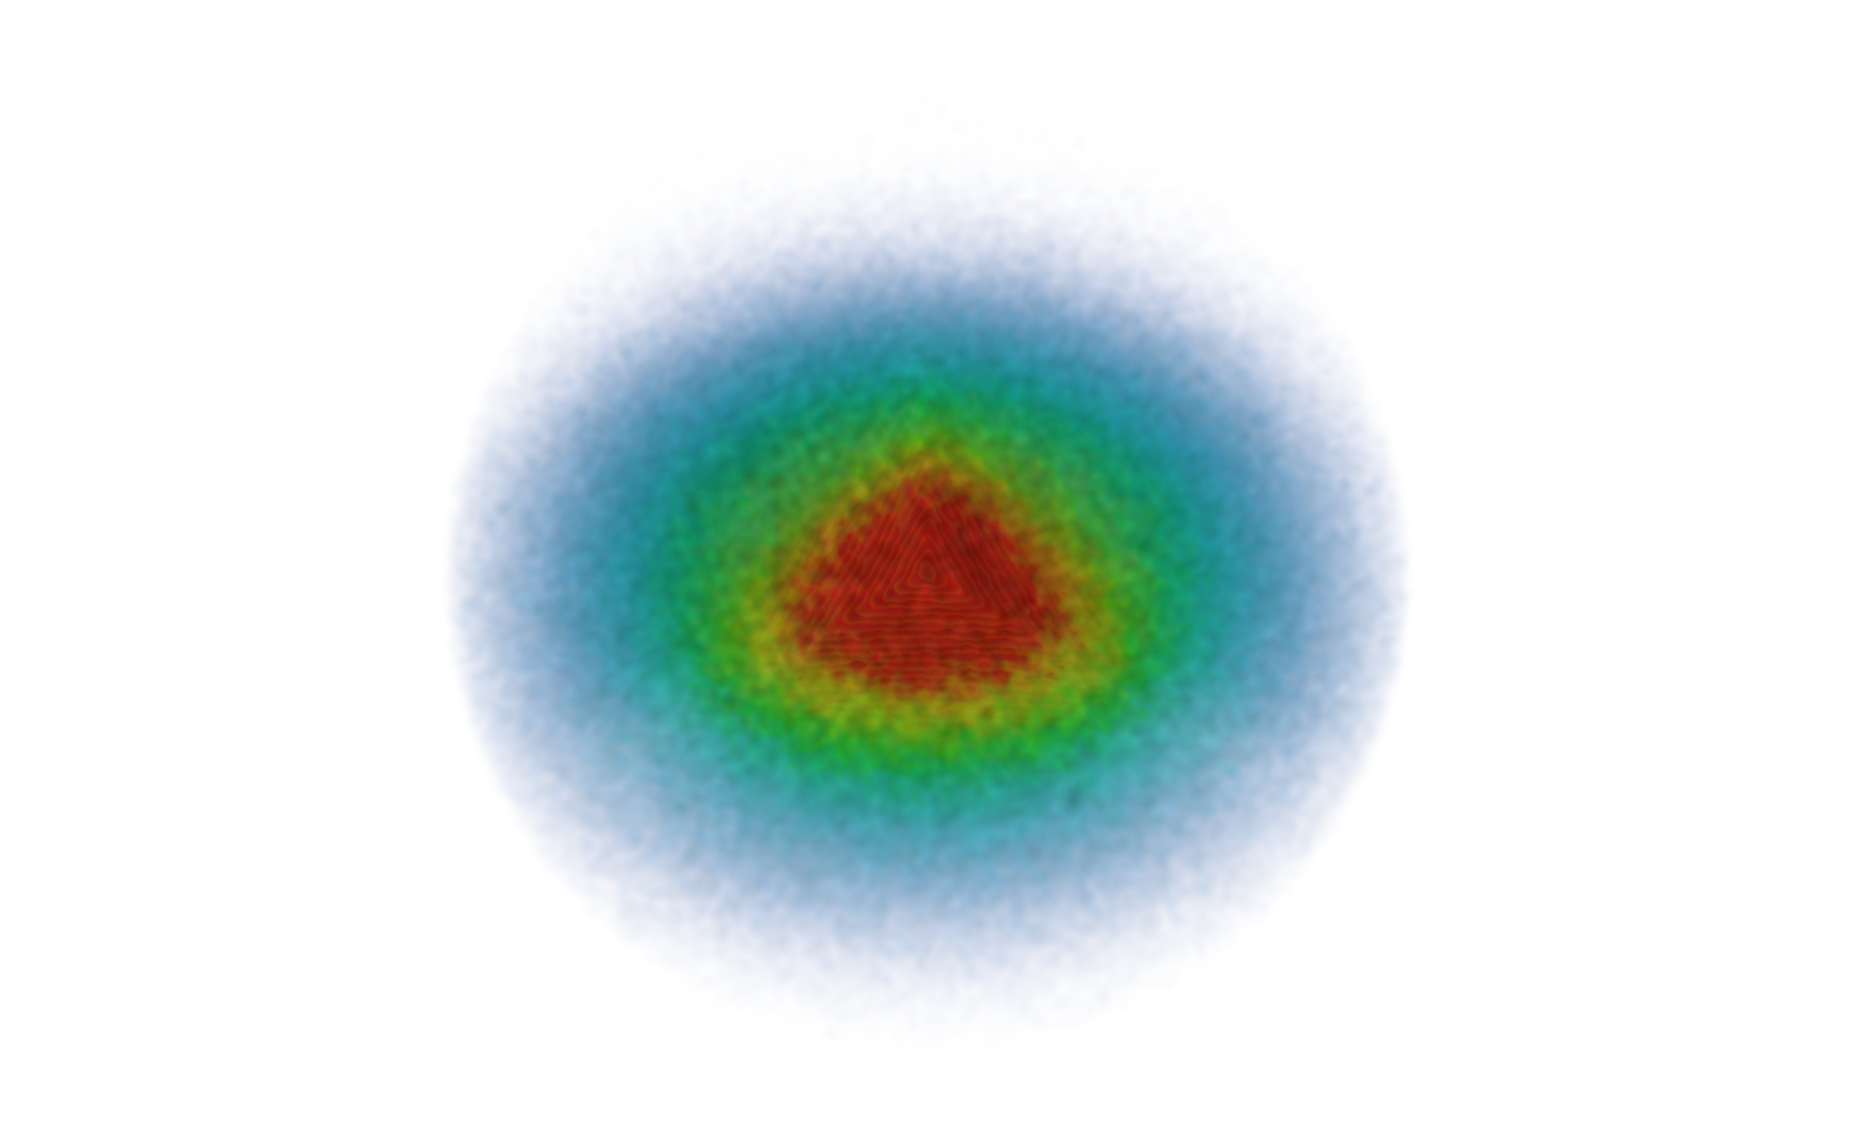
\includegraphics[width=\textwidth]{../modifiedMortenCode/figures/interactingDistribution3.png}
  \caption{}
  \label{fig:minipage1}
\end{minipage}
\quad
\begin{minipage}[t]{0.48\linewidth}
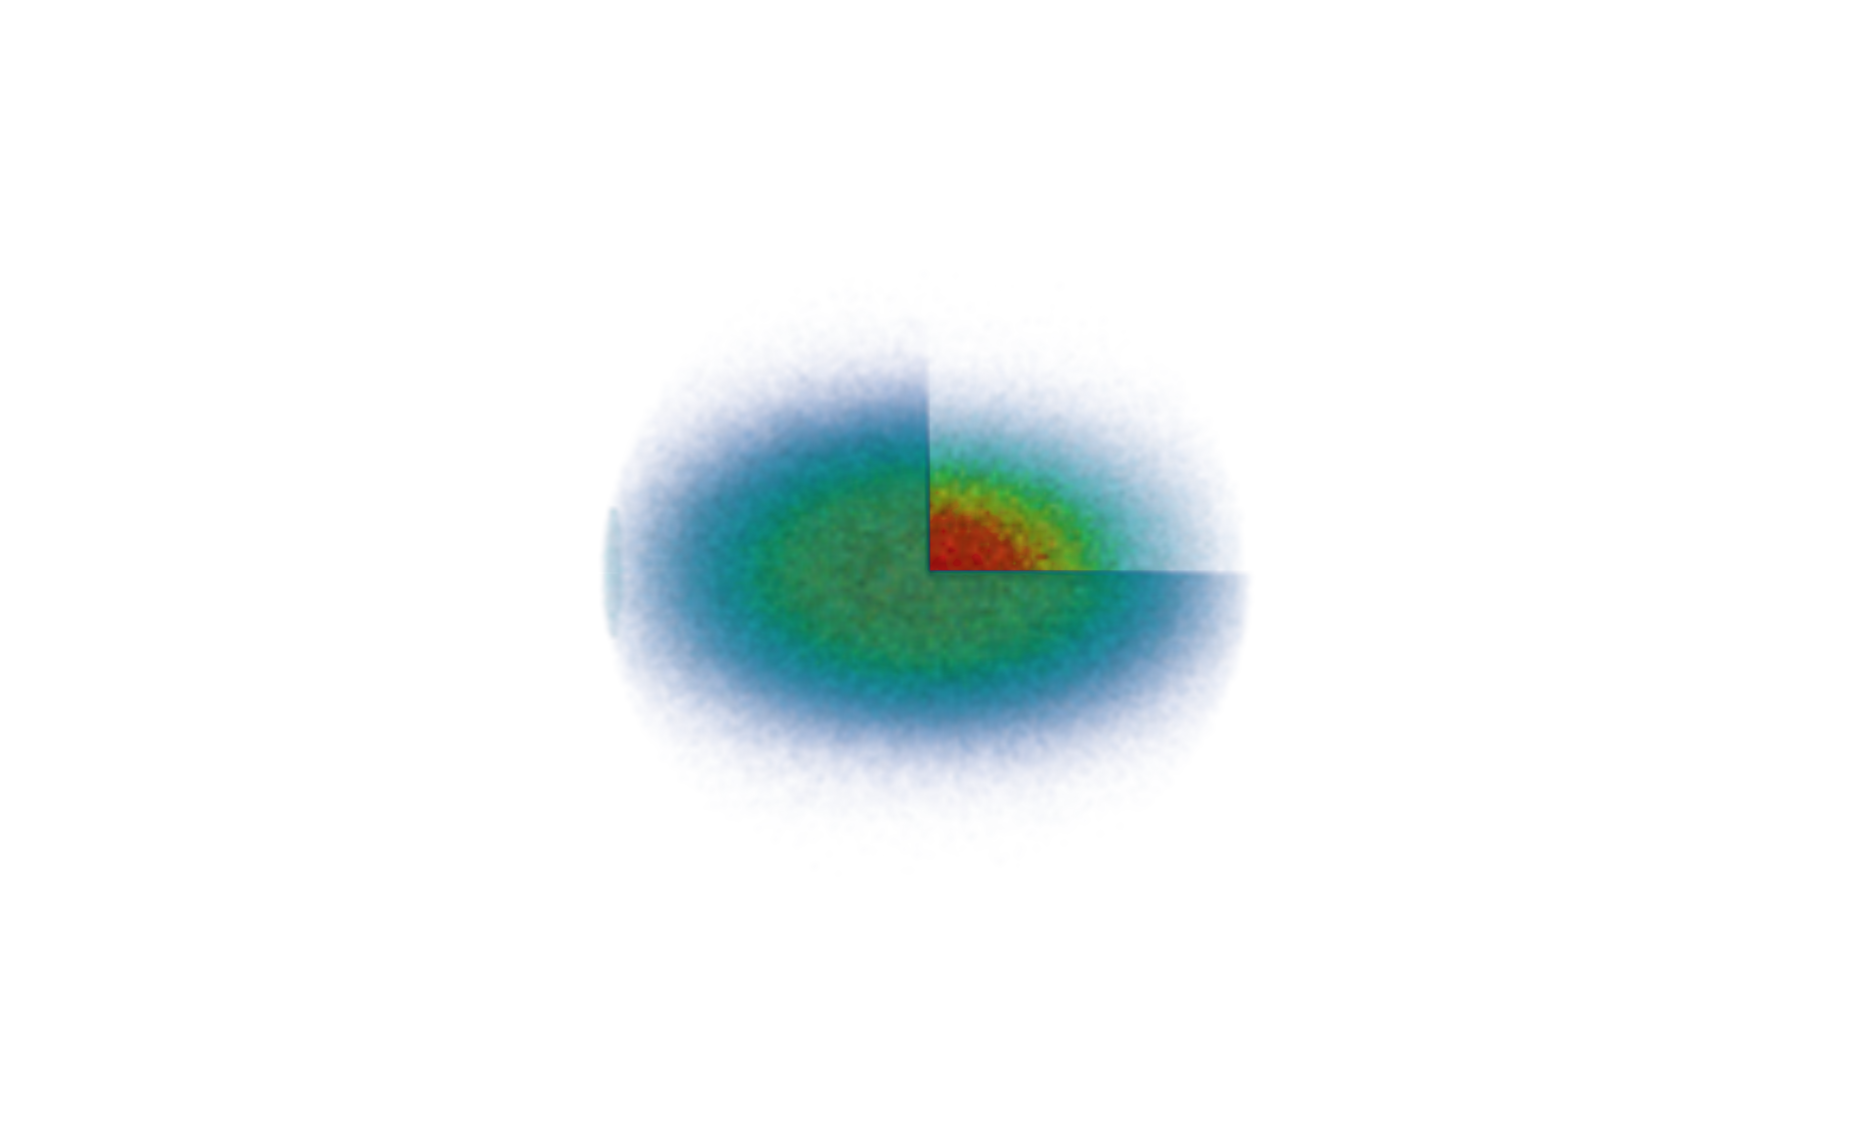
\includegraphics[width=\textwidth]{../modifiedMortenCode/figures/interactingDistributionXZ.png}
  \caption{}
  \label{fig:minipage1}
\end{minipage}
\end{figure}

\section{Conclusions}


\section{Appendix}


 %\end{multicols*}
%%%%%%%%%%%%%%%%%%%%%%%%%%%%%%%%%%%
%%%%%%%%%%%%%%%%%%%%%%%%%%%%%%%%%%%
\end{document}

\begin{comment}

% deloppgave
\begin{enumerate}
\item[\bf a)]
\item[\bf b)]
\item[\bf c)]
\item[\bf d)]
\end{enumerate}

%%%%%%%%
% Tabell
\begin{table}[H]
  \centering
  \begin{tabular}{ | c | r | r | r | r | r |}
    \hline
    & & & & & \\*
    \hline
    & & & & & \\*
    \hline
  \end{tabular}
  \caption{some caption}
  \label{tab:Tabell1}
\end{table}

%%%%%%%%
% Enkel figur
\begin{figure}[H]
\begin{center}
  \includegraphics[width = 120mm]{/users/filiphl/Desktop/Studie/Emne/ObligX/filnavn.png}
  \caption{some caption}\label{fig:fig1}
  \end{center}
\end{figure}

%%%%%%%%
% 2 figurer sbs
\begin{minipage}[t]{0.48\linewidth}
  \includegraphics[width=\textwidth]{fil}
  \caption{}
  \label{fig:minipage1}
\end{minipage}
\quad
\begin{minipage}[t]{0.48\linewidth}
\includegraphics[width=\textwidth]{fil}
  \caption{}
  \label{fig:minipage1}
\end{minipage}
\end{figure}

%%%%%%%%
% X antall kollonner
\begin{multicols*}{X}
\begin{spacing}{0.7} % verticale mellomrom
%kan f.eks benytte align?
\end{spacing}
\end{multicols*}


%%%%%%%%
%Matrise
\begin{equation*}
    {\bf A} = \left(\begin{array}{cccccc}
                           z &z &z &z &z &z \\
                           z &z &z &z &z &z \\
                           z &z &z &z &z &z \\
                           z &z &z &z &z &z \\
                           z &z &z &z &z &z \\
                           z &z &z &z &z &z \\
                      \end{array} \right)
\end{equation*}
%%%%%%%%

